% TEX STUDIO MAGIC-COMMAND
% !TeX document-id = {21ffa6e2-6c8f-4532-897c-386dc477f19a}
% !TeX root = presen.tex
% !TeX encoding = utf8
% !TeX TXS-program:compile = lualatex -synctex=1 -interaction=nonstopmode -halt-on-error %.tex
% !TeX TXS-program:quick = txs:///compile | txs:///view-pdf-internal --embedded
%%%-------------------------------------------------------------------------
%%% PD3プレゼンプレート
%%% 作成: 金沢工大・情報工学科・鷹合研究室
%%%-------------------------------------------------------------------------

% !TeX root = presen.tex
\documentclass[25pt, landscape,oneside]{foils}



% 4:3のスクリーン(古い建物)の場合
%\usepackage[top=15truemm,bottom=22truemm,left=15truemm,right=15truemm,paperwidth=300truemm,paperheight=225truemm]{geometry}

% 16:9のスクリーン(8号館,23号館)の場合
\usepackage[top=15truemm,bottom=22truemm,left=15truemm,right=15truemm,paperwidth=320truemm,paperheight=180truemm]{geometry}


% 箇条書き環境の余白設定
\usepackage[shortlabels]{enumitem}
\setlist[description]{topsep=3mm,parsep=0mm,partopsep=0mm,itemsep=.5\zh,leftmargin=2\zw,labelsep=.5\zw}
\setlist[enumerate]{topsep=3mm,parsep=0mm,partopsep=0mm,itemsep=.5\zh,leftmargin=2\zw,labelsep=.5\zw}
\setlist[itemize]{topsep=3mm,parsep=0mm,partopsep=0mm,itemsep=.5\zh,leftmargin=2\zw,labelsep=.5\zw}


%%%%%%%%%%%%%%%%%%
% フォントの設定
%%%%%%%%%%%%%%%%%%
\usepackage[no-math,deluxe,expert,haranoaji]{luatexja-preset}

\iftrue % 全体的に細身のフォントが良いとき
%\iffalse  % 太めのフォントが良いとき
\setmainfont[BoldFont=HaranoAjiMincho-Bold]{HaranoAjiMincho-Light}
\setsansfont[BoldFont=HaranoAjiGothic-Medium]{HaranoAjiGothic-Light}
\setmainjfont[BoldFont=HaranoAjiMincho-Bold]{HaranoAjiMincho-Light}
\setsansjfont[BoldFont=HaranoAjiGothic-Medium]{HaranoAjiGothic-Light}
\else
\setmainfont[BoldFont=HaranoAjiMincho-Bold]{HaranoAjiMincho-Regular}
\setsansfont[BoldFont=HaranoAjiGothic-Bold]{HaranoAjiGothic-Regular}
\setmainjfont[BoldFont=HaranoAjiMincho-Bold]{HaranoAjiMincho-Regular}
\setsansjfont[BoldFont=HaranoAjiGothic-Bold]{HaranoAjiGothic-Regular}
\fi

\setmonofont{Inconsolata}  % urlやverbatim,listingsなどの欧文フォント

\renewcommand{\kanjifamilydefault}{\gtdefault}  % 日本語フォントをゴシックに
\renewcommand*\familydefault{\sfdefault}
%\mathversion{bold} % 数式フォントを太字に変更する

\usepackage{alltt,upquote,textcomp} % シングル,バッククォートなどの視認性をアップ!
\def\textasciigrave{\char0}

% このパッケージを入れないと verbatim の日本語が何故かゴシックにならない
\usepackage{verbatim}% 


%%%%%%%%%%%%%%%%%%
% PDFの設定
%%%%%%%%%%%%%%%%%%

\usepackage[%
pdfstartview={FitH -32768},%    描画領域の幅に合わせる
bookmarks=true,%                しおり付き
bookmarksnumbered=true,%        章や節の番号をふる
bookmarkstype=toc,%             目次情報のファイル.tocを参照
colorlinks=true,%              ハイパーリンクを色枠に
linkcolor=black,%
urlcolor=black,%
citecolor=black,%
filecolor=black,%
menucolor=black,%
pagecolor=black,%
pdftitle={プロジェクトデザイン3},
pdfsubject={},
pdfauthor={鷹合研究室},
pdfkeywords={},
dvipdfmx-outline-open %%%%%%%%%%%%%%% これがあるとBookmarkを自動的に展開されるみたい・・・
]{hyperref}


%%%%%%%%%%%%%%%%%%%%%%%%%%%
%
% ここから下は必要がない限り書き換えない
%
%%%%%%%%%%%%%%%%%%%%%%%%%%

%%%%%%%%%%%% ブックマークを表示
\usepackage{bookmark}

% スライドの見出しの位置
\setlength{\foilheadskip}{-14mm}

% スライドなので字下げしない
\setlength{\parindent}{0mm}


% ルビ
\usepackage{luatexja-ruby}

\usepackage{bbding} % \PencilRightDown 鉛筆マーク
\usepackage{tikz}
\usepackage[symbol]{footmisc}
\usepackage{xcolor,listings}
\usepackage{multicol}
\usepackage{xurl}
\usepackage{graphicx}
\usepackage{epsfig}

\usepackage{lastpage}
\usepackage{ascmac}
%\usepackage{fancybox,fancyvrb,okumacro}

\renewcommand{\lstlistingname}{List} 

\lstset{%
	language={Python}, 
	backgroundcolor={\color[gray]{.95}},%
	basicstyle={\ttfamily\small},%
	identifierstyle={\ttfamily\small},
	commentstyle={\ttfamily\small\color{red}},
	keywordstyle={\ttfamily\small\color{blue}},
	ndkeywordstyle={},%
	stringstyle={\ttfamily\small\color[rgb]{0,0.5,0}},
	frame={tb},
	breaklines=true,
	columns=[l]{fullflexible},
	%	columns=[l]{fixed},% fixed だと開きすぎ
	basewidth=0.5em,   % これないと行頭のスペースが揃わない
	numbers=left,%
	xrightmargin=0\zw,%
	xleftmargin=3\zw,%
	numberstyle={\ttfamily\small},%
	tabsize=3,
	stepnumber=1, 
	numbersep=0.75\zw,%
	lineskip=-0.3ex,%
	belowcaptionskip=3pt,   % これないと見出しとリスト本体に隙間が毎回変わる
	abovecaptionskip=0pt,
	captionpos=t,
	showstringspaces=false, % 半角スペースを記号で表示しない
}
%

%%%%%%%%%%%% fboxの線幅
\setlength{\fboxrule}{1.5pt}



%%%%%%%%%%%% ページフッタの設定 %%%%%%%%%%%%%
\usepackage{fancyhdr}
\pagestyle{fancy}
\fancyhf{}  % これを入れないと2ページのフッタがずれる
\renewcommand{\headrulewidth}{0pt} % 水平線を消去
\renewcommand{\footrulewidth}{0pt} % 水平線を消去
\renewcommand{\thefootnote}{\fnsymbol{footnote}}

%%%%%%%%%%%%%%%%%%%%%%%%%%%%%%%%%%%%%%
% Verbatim環境にデフォルト値をセット
\usepackage{fancyvrb}
\newenvironment{verbatimx}%
{\small\Verbatim[frame=single,obeytabs,baselinestretch=.65,commandchars=\\\{\}]}%
{\endVerbatim}%

%%%%%%%%%%%%%%%%%%%%%%%%%%%%%%%%%%%%%%
% Verbatim環境にデフォルト値をセット
\newenvironment{myVerbatim}%
{\vspace{-8mm}\Verbatim[frame=single,obeytabs,framesep=2mm,baselinestretch=.7,commandchars=\\\{\}]}%
{\endVerbatim}%


%%%%%%%%%%%%%%%%%%%%%%%%%%%%%%%%%%%%%%
\usepackage{fontawesome5}
\renewcommand{\refname}{文献} % 文献の表記を変更

%%%%%%%%%%%%%%%%%%%%%%%%%%%%%%%%%%%%%%%%%
\renewcommand{\lstlistingname}{リスト}

% 図・表・リストのcaption番号を表示するか/表示しないかを選ぶ
\iffalse
\usepackage[hang,bf,labelformat = empty,labelsep=none,figurename=Y, tablename=X, singlelinecheck=off,justification=centering,labelfont=bf,textfont=bf]{caption} 
\else
\usepackage[hang,bf,labelsep=colon,figurename=図, tablename=表, singlelinecheck=off,justification=centering,labelfont=bf,textfont=bf]{caption} 
\fi

%%%%%%%%%%%%%%%%%%%%%%%%%%%%%%%%%%%%%%%%%
% 
% タイトルスライドのロゴ画像
% フッタ(左)
%%%%%%%%%%%%%%%%%%%%%%%%%%%%%%%%%%%%%%%%%
%  フッタ(左側)

  \MyLogo{
\includegraphics[height=1.1cm]{fig/logo/kit_landscape1.pdf}}
% \MyLogo{--- 鷹合研究室 ---} % トップスライドの下部中央

  \lfoot{
\includegraphics[height=.75cm]{fig/logo/kit_landscape1.pdf}}
% \lfoot{\small 鷹合研}        % フッタ(左)

%%%%%%%%%%%%%%%%%%%%%%%%%%%%%%%%%%%%%%%%%
% 
% フッタ(中央,右)
%
%%%%%%%%%%%%%%%%%%%%%%%%%%%%%%%%%%%%%%%%%
%\cfoot{\thepage/\pageref{LastPage}} 
\cfoot{\thepage/\pageref{LastPage}}
\rfoot{\small 1EP999} % テーマ番号

%%%%%%%%%%%%%%%%%%%%%%%%%%%%%%%%%%%%%%%%%%%
% ページ番号を1からにしたら,トップスライドの下部のロゴがうまくいかなくなったのでこうしてみた
\fancypagestyle{myfirstpage}
{
  \fancyhf{}
   \fancyfoot[C]{
\includegraphics[height=1.1cm]{fig/logo/kit_landscape1.pdf}}
%  \fancyfoot[C]{鷹合研究室}
   \renewcommand{\headrulewidth}{0pt} % removes horizontal header line
}
%%


%%%%%%%%%%%%%%%%%%%%%%%%%%%%%%%%%%%%%%%%%
% 
% ここから下を書き換えて下さい 
%
%%%%%%%%%%%%%%%%%%%%%%%%%%%%%%%%%%%%%%%%%

\title{
{\normalsize 令和98年度 プロジェクトデザインIII}\\\vspace{10mm}
{\LARGE WebAssemblyを用いた\\グラフィクスレンダリングの高速化}
}
\date{令和99年99月99日}
\author{
4EP5-04\\ \ruby{天羽}{あもう}\ruby{大樹}{たいき}
}



\begin{document}
\maketitle % タイトルページ
\addtocounter{page}{1}
\thispagestyle{myfirstpage}

%%%%%%%%%%%%%%%%%%%%%%%%%%%%%
 \foilhead{\Large 1. はじめに -- 背景と目的 -- }
\begin{itemize}
 \item 将来、Webアプリケーションとして、リアルタイムに変化するxRコンテンツを作成し、動作させる際、グラフィクスレンダリングの速度が遅くなってしまうと、没入感を損なってしまう問題があると考えられる
 \item そのような問題に対処するために、Web上でグラフィクスのレンダリングを早く処理するために、どのような手法を用いれば、より早く処理できるのかという取り組みを行う必要がある
 \item 本プロジェクトにおいては、WebAssemblyという仕組みを用いたバイナリフォーマットプログラムを使って、グラフィクスレンダリングを早く処理させるプログラムを作成する
\end{itemize}
\newpage

%%%%%%%%%%%%%%%%%%%%%%%%%%%%%
\foilhead{\Large 発表の流れ}
\begin{enumerate}[itemsep=0.25\zh]
	\item \textcolor{gray}{はじめに -- 背景と目的 --}
	\item 用語などの簡潔な説明
	\item プログラム概要
	\item 評価
	\item むすび
\end{enumerate}
\newpage

%%%%%%%%%%%%%%%%%%%%%%%%%%%%%%%%%%%%%%%%%%%%%%
\foilhead{\Large 2. 用語の簡潔な説明}
\begin{itemize}
	\item WebAssembly\\Web上で動作するバイナリフォーマットプログラムのこと。\\wasmと略して呼称されることが多いため、本スライドでも\\その略称を以後使用する。特定のプログラミング言語で記述した\\プログラムをそのバイナリフォーマットにコンパイルしたものを\\主に指す。そのプログラムを保存したファイルは、\\wasmモジュールと呼称されることが多い。
	\newpage
	
	\item WebGL\\Web上でグラフィクスを扱うために、ブラウザに組み込まれているAPI\\後述するWebGPUより歴史が古く関連ライブラリが豊富で、\\Three.jsやBabylon.jsといったライブラリが有名。
	
	\item WebGPU\\WebGLより高度にGPUの性能を活かし、高速なグラフィクス\\レンダリングを行うことが可能であるとされている\\ブラウザ組み込みのAPI。まだ公開されてから日が浅いため、\\著名な関連ライブラリなどはまだあまり見受けられない
\end{itemize}

%%%%%%%%%%%%%%%%%%%%%%%%%%%%%%%%%%%%%%%%%%%%%%
\foilhead{\Large 3. プログラム概要}


ここにブロック図をいれシステム全体を解説する.ドローンや車両などを開発した場合は,その写真も示す.
%% \begin{figure}[h]
%% \begin{center}
%% 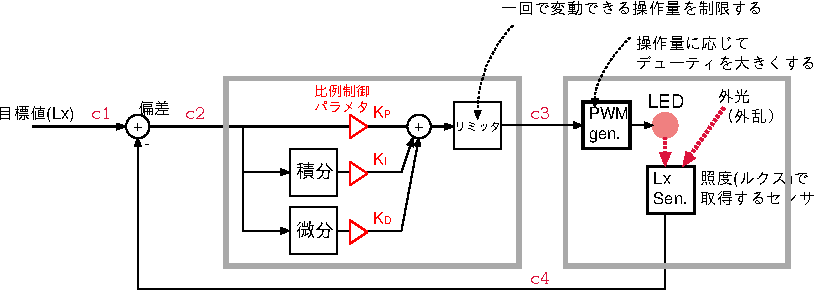
\includegraphics[width=\textwidth]{fig/system.pdf}
%% \caption{}
%% \end{center}
%% \end{figure}
\newpage

%%%%%%%%%%%%%%% minipage の利用例 %%%%%%%%%%%%%%%%%%%
%------ 左側
\begin{minipage}[t]{0.4\textwidth}\vspace{0pt}
あああああああああああああああああああああああああああああああああああああああああああああああああああああああああいゆえお.
\begin{itemize}[parsep=-0.5\zh]
	\item いいいいいいいいいいいいいいいいい
	\item うううううううううううううううううう
	\item えええええええええええええええええええええええええ
\end{itemize}
\end{minipage}
%------ 右側
\begin{minipage}[t]{0.6\textwidth}\vspace{0pt}
\begin{center}
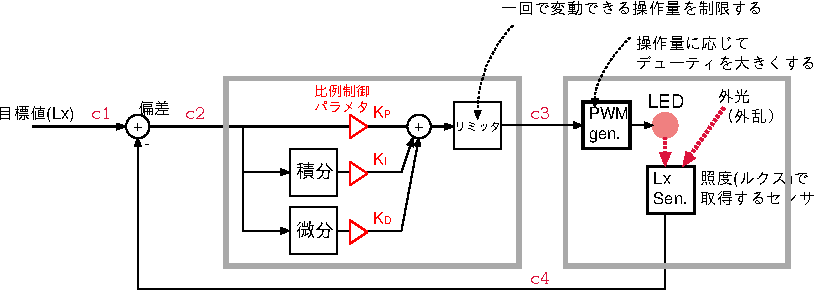
\includegraphics[keepaspectratio, width=.9\linewidth,trim={100mm 0mm 0mm 15mm},clip]{fig/system.pdf}
\end{center}
\end{minipage}

%%%%%%%%%%%%%%%%%%%%%%%%%%%%%%%%%%%%%%%%%%%%%%
\foilhead{\Large 3-1. 畳み込みニューラルネットワークの構造}
\begin{description}
	\item[①入力層]~\\
	ああああああああああああああああああああああいいいいいいいいいいいいいいいいいいいいいいいいいいいいいいいいいいいいいいいうううううううううううううううう
	\item[②中間層]~\\
	ああああああああああああああああああああああいいいいいいいいいいいいいいいいいいいいいいいいいいいいいいいいいいいいいいいうううううううううううううううう
	\item[③出力層]~\\
	あああああああ\textcolor{red}{ああああああああ}あああああ
	\begin{enumerate}
		\item 巧言令色,鮮なし仁
		\item 後生畏可し,焉んぞ来者の今に,如かざるを知らんや.
	\end{enumerate}
\end{description}
\newpage

%%%%%%%%%%%%%%%%%%%%%%%%%%%%%%%%%%%%%%%%%%%%%%
\foilhead{\Large 3-2. ○○○○○処理の方法}
\begin{description} 
	\item[①Javascript]~\\
	ああああああああああああああああああああああいいいいいいいいいいいいいいいいいいいいいいいいいいいいいいいいいいいいいいいうううううううううううううううう
	\item[②Python+Tornado]~\\
	ああああああああああああああああああああああいいいいいいいいいいいいいいいいいいいいいいいいいいいいいいいいいいいいいいいうううううううううううううううう
	\item[③pigpio]~\\
	ああああああああああああああああああああああいいいいいいいいいいいいいいいいいいいいいいいいいいいいいいいいいいいいいいいうううううううううううううううう
\end{description}
\newpage


%%%%%%%%%%%%%%%%%%%%%%%%%%%%%%%%%%%%%%%%%%%%%%
\foilhead{\Large 4. 評価・考察}
\begin{itemize}
	\item このスライドでは何をどのような方法で評価したかを明記し,結果をグラフで示すこと(表よりグラフのほうが良い).
	\item システムが動いている様子がわかるようにデモ映像を流すこと(デモ映像には字幕をつけたりするなどしてわかりやすくすること).
	\item 評価の際は,改良の前後でどうなったかを示す.あるいは他の手法などと比較してどうなのかを示すことも必要.
	\item 結果について考察も示すこと.
\end{itemize}
\newpage

%%%%%%%%%%%%%%%%%%%%%%%%%%%%%%%%%%%%%%%%%%%%%%
\foilhead{\Large 5. むすび}\label{MUSUBI}
\begin{itemize}
	\item 何のために何を作成したかを改めて書く.
	\item 現時点での評価結果,考察を簡潔に書く.
	\item 来月の報告までに何をするか計画を書く.
\end{itemize}
\newpage

%%%%%%%%%%%%%%%%%%%%%%%%%%%%%%%%%%%%%
ここからおまけ

\href{run:./demo002.mp4}{\textcolor[hsb]{0.0, 0.7, 1.0}{\faPlayCircle[regular]}} PDFファイルと同じフォルダにdemo002.mp4があれば再生できる.


\href{https://youtu.be/74agBeJxdFI}{\textcolor{red}{\faYoutube}} YOUTUBEで再生

\textcolor{red}{\faYoutube}\href{https://youtu.be/74agBeJxdFI}{~\url{https://youtu.be/74agBeJxdFI}}

\lstinputlisting[language=c, caption=test2.c]{src/hello.c}
\lstinputlisting[language=python, caption=test2.py]{src/world.py}

% 色定義
\definecolor{mygray}{gray}{0.95}
\definecolor{mypink1}{hsb}{0.0, 0.188, 1.0}
UNIXv1におけるタスク切り替えが行われるタイミング

%%%%%%%%%%%%%%%%%%%%%%%%55
\colorbox{mygray}{\begin{minipage}{\textwidth}
① みなさん
\end{minipage}}

\colorbox{mygray}{\begin{minipage}{\textwidth}
② こんにちは 
\begin{itemize}
\item まんじゅう
\item りんご
\end{itemize}
\end{minipage}}

\colorbox{mypink1}{\begin{minipage}{\textwidth}
③ お元気で\\
またあうひまで
\end{minipage}}
%%%%%%%%%%%%%%%%%%%%%%%%%%%%%%%%%%%%%%%%%%%%

\begin{verbatimx}
$ gcc test.c \return
 (*_*)
 (*_*)
        \textcolor{red}{ここで\keytop{CTL}+\keytop{C}を押す}
\end{verbatimx}
%%%%%%%%%%%%%%%%%%%%%%%%%%%%%%%%%%%%%%%%%%%%%%%%%%%%%%%%%%%%%%%%%%%%%%%%
\newpage
~\\
\noindent\textbf{謝辞}~~本研究はJSPS科研費21Kxxxxxxxxx助成を受けた
%%%%%%%%%%%%%%%%%%%%%%%%%%%%%% 参考文献 %%%%%%%%%%%%%%%%%%%%%%%%%%%%%%
\begin{thebibliography}{99}
\small
\setlength\itemsep{-0.5\zh}%
\bibitem{book1} K.Thompson,D.M.Ritchie,\textbf{"The UNIX Time-Sharing System"},Communications of the ACM, Vol.17, No.7, 1974.
\bibitem{book4} Digital Equipment Corporation: \textbf{PDP11/20-15-r20 Processor Handbook}, 1971.
\bibitem{Preliminary} T.R. Bashkow, \textbf{"Study of UNIX: Preliminary Release of Unix Implementation Document"}, \url{ http://minnie.tuhs.org/Archive/Distributions/Research/Dennis_v1/PreliminaryUnixImplementationDocument_Jun72.pdf}, Jun. 1972.
%\bibitem{book2} K. Thompson,D.M. Ritchie,"UNIX PROGRAMER'S MANUAL",Nov. 1971.
%\bibitem{web0} Warren Toomey, "The Unix Heritage Society", \url{https://www.tuhs.org/}, Dec. 2015.
\bibitem{simh} simh, \textbf{"The Computer History Simulation Project"}, \url{https://github.com/simh/simh}, 参照Mar.14, 2022.
\bibitem{ref0} W.Toomey, \textbf{"First Edition Unix: Its Creation and Restoration"}, IEEE Annals of the History of Computing, 32 (3), pp.74-82, 2010.
%\bibitem{web1} Jim Huang, "Restoration of 1st Edition UNIX from Bell Laboratories", \url{https://github.com/jserv/unix-v1}, 参照Mar.14, 2022.
\bibitem{book3} Diomidis.Spinellis,\textbf{"unix-history-repo"},  \url{https://github.com/dspinellis/unix-history-repo/tree/Research-V1}, 参照Mar.14, 2022.
\bibitem{book5} Digital Equipment Copporation: \textbf{PDP11 Peripherals HandBook}, 1972.
%\bibitem{book6} \url{https://github.com/No000/unix-v1-utils}
%\bibitem{book7} \url{https://github.com/No000/UnixV1-SystemCallTracer}
\end{thebibliography}

\end{document} 
